\documentclass[12pt,a4paper,titlepage]{article}
\usepackage[pdftex]{graphicx}
\usepackage[polish]{babel}
\usepackage[utf8]{inputenc}
\usepackage[T1]{fontenc}
\usepackage{tabularx}
\usepackage{tikz}
\usepackage{tikz-qtree}

\renewcommand{\labelenumii}{\arabic{enumi}.\arabic{enumii}}
\renewcommand{\labelenumiii}{\arabic{enumi}.\arabic{enumii}.\arabic{enumiii}}
\renewcommand{\labelenumiv}{\arabic{enumi}.\arabic{enumii}.\arabic{enumiii}.\arabic{enumiv}}

\tikzset{every tree node/.style={align=center,anchor=north}}

\title{Prover - automatyzacja procesu wnioskowania logicznego z wykorzystaniem drzew prawdy}
\author{Stanisław Maciąg, Piotr Mitana}
\date{2014}



\begin{document}
\newcolumntype{L}[1]{>{\raggedright\arraybackslash}p{#1}}
\newcolumntype{C}[1]{>{\centering\arraybackslash}p{#1}}
\newcolumntype{R}[1]{>{\raggedleft\arraybackslash}p{#1}}

\maketitle

\section{Założenia projektowe}
W ramach projektu zaprojektowana oraz zaimplementowana zostanie aplikacja, realizująca proces wnioskowania na podstawie dostarczonych przez użytkownika formuł logicznych stanowiących przesłanki oraz konkluzje. Poprawność wnioskowania sprawdzana będzie z wykorzystaniem algorytmu operującego na drzewach prawdy (ang. \textit{Truth Trees}).

\subsection{Środowisko}
\begin{enumerate}
	\item System operacyjny Linux
	\item Języki programowania C++ oraz D
\end{enumerate}

\subsection{Implementowane funkcjonalności}
\begin{enumerate}
	\item Graficzny interfejs użytkownika (\textit{GUI}), umożliwiający wygodną obsługę aplikacji
	\item Dane wejściowe (formuły logiczne) wprowadzane ręcznie w postaci ciągu znaków, lub z pliku tekstowego (składnia wyrażeń opisana w \ref{skladnia})
	\item Zapis danych wejściowych, otrzymanego drzewa prawdy oraz wyniku do pliku
	\item Wizualizacja drzewa prawdy
\end{enumerate}

\section{Analiza leksykalna}

\subsection{Składnia formuły wejściowej}
\label{skladnia}
\begin{tabular}{|C{5cm}|C{5cm}|}
  \hline
  \textbf{Ciąg znaków} & \textbf{Znaczenie}\\ 
  \hline 
  Ciąg znaków alfanumerycznych & Zmienna logiczna rozumiana jako formuła atomowa\\
  \hline
  ![formuła] & Jednoargumentowy operator negacji\\
  \hline
  [formuła] \& [formuła] & Dwuargumentowy operator koniunkcji logicznej\\
  \hline
  [formuła] | [formuła] & Dwuargumentowy operator alternatywy logicznej\\
  \hline
  [formuła] \^{} [formuła] & Dwuargumentowy operator alternatywy wykluczającej\\
  \hline
  [formuła] > [formuła] & Dwuargumentowy operator implikacji logicznej\\
  \hline
  [formuła] = [formuła] & Dwuargumentowy operator ekwiwalencji logicznej\\
  \hline
  ([formuła]) & Nawiasy okrągłe - grupowanie wyrażeń\\
  \hline
\end{tabular}

\subsection{Hierarchia operatorów}
\begin{tabular}{|C{5cm}|C{5cm}|}
  \hline
  \textbf{Operator} & \textbf{Priorytet}\\
  \hline
  Negacja & Najwyższy\\
  \hline
  Koniunkcja, alternatywa, alternatywa wykluczająca & Średni\\
  \hline
  Implikacja, Ekwiwalencja & Najniższy\\
  \hline
\end{tabular}

\subsection{Reguły wydzielania tokenów}
\begin{enumerate}
	\item Białe znaki rozdzielające tokeny są ignorowane, jednak ich wystąpienie powoduje natychmiastowe odcięcie tokena od reszty formuły (w wypadku poprawnej składniowo formuły nie wpłynie to na sposób jej podziału)
	\item Nawiasy oraz operator negacji są samodzielnymi tokenami, więc są natychmiastowo odcinane i zwracane
	\item Ciąg znaków niealfanumerycznych (z wyłączeniem białych znaków, nawiasów i wykrzyknika) zostanie zwrócony jako jeden token (operator)
	\item Ciąg znaków alfanumerycznych zostanie zwrócony jako jeden token (zmienna)
\end{enumerate}

\subsection{Reguły walidacji}
Definiowane są w następujący sposób – dla każdego elementu składniowego określane jest, czy może stać na początku oraz jakie elementy dozwolone są za nim.

\begin{tabular}{|C{3cm}|C{3cm}|C{5cm}|}
\hline
\textbf{Element języka} & \textbf{Może zaczynać formułę} & Dozwolone następne tokeny\\
\hline
Zmienna logiczna & Tak & \&, |, \^{}, >, =, ), koniec formuły\\
\hline
! & Tak & Zmienna logiczna, !, (\\
\hline
\&, |, \^{}, >, = & Nie & Zmienna logiczna, !, (\\
\hline
( & Tak & Zmienna logiczna, !, (\\
\hline
) & Nie & \&, |, \^{}, >, =, ), koniec formuły\\
\hline
\end{tabular}

Dodatkowo, ilości nawiasów otwierających i zamykających muszą być równe.
\newpage

\section{Algorytm działania}

\begin{figure}[!htb]
\centering
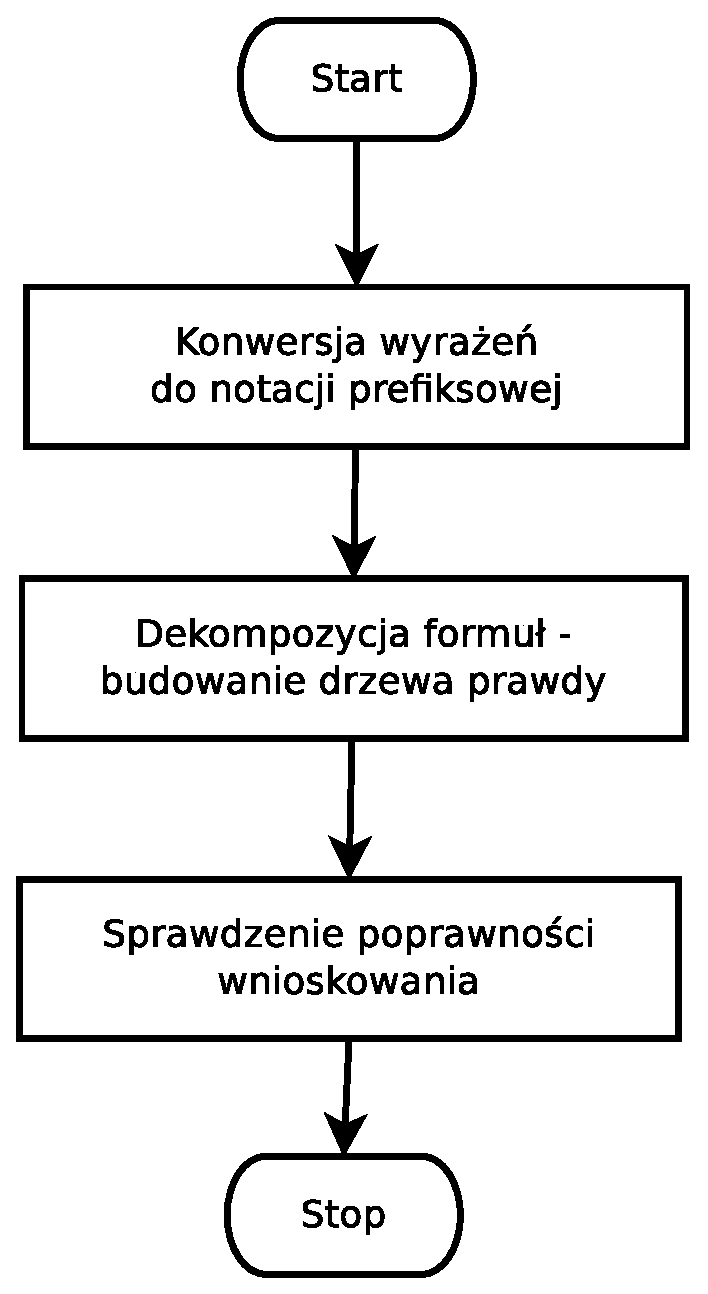
\includegraphics[height=7cm]{main_alg}
\caption{Przebieg głównego algorytmu}
\end{figure}

\subsection{Konwersja do notacji prefiksowej}
Przed procesem dekompozycji formuła zostaje przetworzona do postaci prefiksowej (będącej de facto prostą reprezentacją drzewa), w której tokeny oddzielone są pojedynczą spacją. Proces ten należy poprzedzić walidacją formuły, ponieważ funkcja budująca drzewo już zakłada jej poprawność.

\subsubsection{Walidacja}
Proces walidacji polega na sprawdzeniu sąsiedztwa każdego z tokenów zgodnie z regułami podanymi wcześniej. Faktycznie są one jednak sprawdzane pośrednio – funkcja walidująca sprawdza poprzedzający operator, a nie następny (słowo a może stać przed słowem b wtedy i tylko wtedy, gdy słowo b może stać za słowem a). Dodatkowe reguły:
\begin{itemize}
	\item Na początku procesu zmienna przechowująca poprzedni token jest pusta – sprawdzenie, czy dany token może zaczynać formułę sprowadzone jest do sprawdzenia, czy może być poprzedzone przez pusty token
	\item Koniec formuły wykryty jest, gdy zostanie wczytany pusty token. Następuje więc sprawdzenie, czy pusty token może być poprzedzane przez poprzedni (będący ostatnim w formule)
	\item Na końcu procesu walidacji sprawdzany jest balans nawiasów
\end{itemize}

\subsubsection{Algorytm konwersji}
Proces ten dokonywany jest przy użyciu dwóch stosów – operatorów oraz operandów. Stosy są reprezentowane przez ciągi znaków, których elementy oddzielone są tabulacjami. Poniżej wypisane są kroki algorytmu.
\begin{enumerate}
	\item Pobieraj kolejne słowa formuły, dla każdego wykonaj:
	\begin{enumerate}
		\item Jeżeli „(”, odłóż na stos operatorów
		\item Jeżeli „)”, to:
		\begin{enumerate}
			\item Zdejmuj ze stosu operatorów tak długo, aż napotkasz „(”
			\item Dla każdego operatora zdejmij właściwą ilość argumentów ze stosu operandów Odłóż na stos operandów wartość zawierającą operator oraz jego argumenty oddzielone spacjami
		\end{enumerate}
		\item Jeżeli inny operator (przyjmijmy \textit{a}), to:
		\begin{enumerate}
			\item Zdejmuj ze stosu operatorów (przyjmijmy \textit{b}), dopóki operator \textit{b} ma taki sam lub większy priorytet od \textit{a}. Dla każdego wykonaj:
			\begin{enumerate}
				\item Zdejmij właściwą dla operatora ilość argumentów ze stosu operandów
				\item Odłóż na stos operandów wartość zawierającą operator oraz jego argumenty oddzielone spacjami
			\end{enumerate}
			\item Odłóż \textit{b} na stos operatorów (\textit{b} będzie pierwszym o priorytecie mniejszym od \textit{a})
			\item Odłóż \textit{a} na stos operatorów
		\end{enumerate}
		\item W innym wypadku (czyli nazwa zmiennej) odłóż na stos operandów
	\end{enumerate}
	\item Pobierz i zwróć wynik ze stosu operandów
\end{enumerate}

\subsection{Dekompozycja formuły}

\subsubsection{Drzewa prawdy}
Drzewa prawdy stanowią jedno z narzędzi służących do rozwiązywania problemów logicznych. Ich główną zaletą jest duża efektywność, przekładająca się na mniejszą złożoność czasową. Metody wykorzystujące drzewa prawdy nie wymagają rozwiązywania trudnych problemów decyzyjnych, dzięki czemu są dobrze algorytmizowalne. Poniżej przedstawiono listę problemów, które można rozwiązać korzystając z drzew prawdy:

\begin{itemize}
	\item Dowodzenie sprzeczności lub niesprzeczności zbioru twierdzeń
	\item Sprawdzanie poprawności dowodu (wnioskowania)
	\item Wykrywanie tautologii i kontrtautologii
	\item Sprawdzenie semantycznej równoważności
\end{itemize}

Bez względu na charakter analizowanego problemu, rozwiązanie zawsze uzyskuje się w trzech następujących krokach:

\begin{enumerate}
	\item Zdefiniowanie korzenia drzewa, zgodnie z typem rozpatrywanego problemu
	\item Budowanie drzewa poprzez zastosowanie reguł dekompozycji do złożonych wyrażeń logicznych (przedstawione w \ref{dekompozycja}
	\item Interpretacja wyników
\end{enumerate}

\subsubsection{Reguły dekompozycji}
\label{dekompozycja}

\begin{tabular}{|C{5cm}|C{5cm}|}
\hline
\textbf{Postać dekompozycji} & \textbf{Nazwa}\\
\hline
\Tree [.{$p \wedge q$} [.{$p$ \\ $q$} ] ] &  Koniunkcja\\
\hline
\Tree[.{$p \vee q$} {$p$} {$q$} ] &  Alternatywa\\
\hline
\Tree[.{$p \Rightarrow q$} {$\neg p$} {$q$} ] &  Implikacja\\
\hline
\Tree[.{$p \Leftrightarrow q$} {$p$ \\ $q$} {$\neg p$ \\ $\neg q$} ] &  Ekwiwalencja\\
\hline
\Tree [.{$\neg(p \wedge q)$} {$\neg p$} {$\neg q$} ] &  Negacja koniunkcji\\
\hline
\Tree [.{$\neg(p \vee q)$} [.{$\neg p$ \\ $\neg q$} ] ] &  Negacja alternatywy\\
\hline
\Tree [.{$\neg(p \Rightarrow q)$} [.{$p$ \\ $\neg q$} ] ] &  Negacja implikacji\\
\hline
\Tree[.{$\neg(p \Leftrightarrow q)$} {$p$ \\ $\neg q$} {$\neg p$ \\ $q$} ] &  Negacja ekwiwalencji\\
\hline
\Tree [.{$\neg \neg p$} [.{$p$} ] ] &  Negacja negacji\\
\hline
\end{tabular}

\subsubsection{Algorytm sprawdzania poprawności dowodu}
\begin{enumerate}
	\item Tworzenie korzenia drzewa poprzez zapis przesłanek oraz \textit{zaprzeczenia} konkluzji w postaci ciągu wyrażeń (kolumny) o numerowanych (rozróżnialnych) wierszach
	\item Dekompozycja następnego w kolejności wyrażenia logicznego. Kolejność dekomponowania wyrażeń znajdujących się w węzłach drzewa jest dowolna, jednak ze względu efektywność algorytmu najlepiej przyjąć następujący porządek:
	\begin{itemize}
	\item[1] Dekomponowanie wyrażeń niepowodujących rozgałęziania - koniunkcja, zaprzeczenie alternatywy oraz zaprzeczenie implikacji
	\item[2] Dekomponowanie wyrażeń powodujących rozgałęzianie oraz tworzących dwa pod-wyrażenia w węzłach potomnych - ekwiwalencja oraz zaprzeczenie ekwiwalencji
	\item[3] Dekomponowanie wyrażeń powodujących rozgałęzianie oraz tworzących jedno wyrażenie w węzłach potomnych - zaprzeczenie koniunkcji, alternatywa, implikacja
	\end{itemize}
	\item Dekompozycję powtarza się, dopóki w liściach drzewa nie pozostaną same pojedyncze zmienne logiczne bądź ich zaprzeczenia
	\item Zamykanie gałęzi - gałąź drzewa określa się jako zamkniętą, jeśli na ścieżce od korzenia drzewa do liścia występuje pojedyncza zmienna logiczna oraz jej zaprzeczenie
	\item Interpretacja wyników - jeżeli drzewo posiada przynajmniej jedną otwartą gałąź to wnioskowanie jest niepoprawne
\end{enumerate}

\subsubsection{Programowa realizacja dekompozycji wyrażeń}
W zastosowanym przez nas algorytmie postać prefiksowa zostanie przekształcona do postaci właściwego drzewa, którego węzły będą przechowywały tablice napisów zawierające kolejne zdania logiczne w postaci prefiksowej. Poniżej zaprezentowano fragment algorytmu wykonujący jeden krok dekompozycji pojedynczej formuły:
\begin{enumerate}
	\item Jeżeli słowo jest zmienną, wróć
	\item Jeżeli jest operatorem negacji, pobierz następne słowo (będzie operatorem) i połącz z poprzednim
	\item Każdy z argumentów operatora pobierz w następujący sposób:
	\begin{enumerate}
		\item Ustal ilość wymaganych symboli na 1
		\item Pobieraj kolejny symbol, dopóki ilość wymaganych symboli jest większa od 0. Dla każdego wykonuj:
		\begin{enumerate}
			\item Jeżeli symbol jest zmienną, zmniejsz ilość wymaganych symboli o 1
			\item Jeżeli symbol jest operatorem, zwiększ ilość wymaganych symboli o ilość argumentów tego operatora - 1
		\end{enumerate}
		\item Argumentem są wszystkie pobrane symbole w kolejności ich występowania
	\end{enumerate}
	\item Zgodnie z regułami dekompozycji utwórz jeden lub dwa węzły potomne i przypisz im odpowiednie wartości
\end{enumerate}
\end{document}